% --------------------------------------------------------------
% This is all preamble stuff that you don't have to worry about.
% Head down to where it says "Start here"
% --------------------------------------------------------------
 
\documentclass[12pt]{article}
 \listfiles
\usepackage[margin=1in]{geometry} 
\usepackage{amsmath,amsthm,amssymb,mathtools}
\usepackage{float}
\usepackage{graphicx}
\usepackage{cancel}
\usepackage{tikz}
\usepackage{xcolor}
\usepackage{bm}

\usepackage{pgfplots}
%\pgfplotsset{compat=1.10}
\usetikzlibrary{intersections}
%\usepgfplotslibrary{fillbetween}

\newcommand{\N}{\mathbb{N}}
\newcommand{\Z}{\mathbb{Z}}
\newcommand{\sign}[1]{\text{sign}(#1)}
\newcommand{\abs}[1]{\left| #1 \right|}
\newcommand{\BigO}[1]{\mathcal{O}\left( #1 \right)}
\renewcommand{\Pr}[1]{\text{Pr}[ #1 ]}
 
\newenvironment{theorem}[2][Theorem]{\begin{trivlist}
\item[\hskip \labelsep {\bfseries #1}\hskip \labelsep {\bfseries #2.}]}{\end{trivlist}}
\newenvironment{lemma}[2][Lemma]{\begin{trivlist}
\item[\hskip \labelsep {\bfseries #1}\hskip \labelsep {\bfseries #2.}]}{\end{trivlist}}
\newenvironment{exercise}[2][Exercise]{\begin{trivlist}
\item[\hskip \labelsep {\bfseries #1}\hskip \labelsep {\bfseries #2.}]}{\end{trivlist}}
\newenvironment{problem}[2][Problem]{\begin{trivlist}
\item[\hskip \labelsep {\bfseries #1}\hskip \labelsep {\bfseries #2.}]}{\end{trivlist}}
\newenvironment{question}[2][Question]{\begin{trivlist}
\item[\hskip \labelsep {\bfseries #1}\hskip \labelsep {\bfseries #2.}]}{\end{trivlist}}
\newenvironment{corollary}[2][Corollary]{\begin{trivlist}
\item[\hskip \labelsep {\bfseries #1}\hskip \labelsep {\bfseries #2.}]}{\end{trivlist}}
 
\begin{document}
 
% --------------------------------------------------------------
%                         Start here
% --------------------------------------------------------------
 
\title{Homework 1}%replace X with the appropriate number
\author{Christopher Mertin\\ %replace with your name
CS6966: Theory of Machine Learning} %if necessary, replace with your course title
 
\maketitle

\begin{enumerate}
\item Consider the problem of classifying points in the two-dimensional plane, {\em i.e.}, $\chi = \mathbb{R}^{2}$. Suppose that the (unknown) true label of a point $(x,y)$ is given by $\sign{x}$ (we define $\sign{0} = \pm 1$ for convenience). Suppose the input distribution $\mathcal{D}$ is the uniform distribution over the unit circle centered at the origin.

\begin{enumerate}
\item Consider the hypothesis $h$ as shown in the figure below ($h$ classifies all the points on the right of the line as $+1$ and all the points to the left as $-1$). Compute the risk $L_{\mathcal{D}}(h)$, as a function of $\theta$ (which is, as is standard, given in radians). 

\begin{figure}[H]
\centering
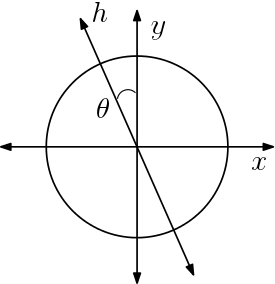
\includegraphics[width=.25\textwidth]{hw1_fig1.png}
\end{figure}

{\bf Solution:}

\begin{align*}
Area_{circle} &= \pi r^{2}\\
Area_{slice} &= \cancel{\pi} r^{2} \frac{\theta}{2\cancel{\pi}} = \frac{\theta }{2}r^{2}\\
\intertext{For a unit circle, the failure percentage for some uniform random distribution on the unit circle $(r = 1)$ would be for two slices}
\mathcal{L}_{\mathcal{D}}(h) &= \frac{\theta r^{2}}{\pi r^{2}} = \frac{\theta}{\pi}
\end{align*}

\item Suppose we obtain $1/\theta$ (which is given to be an integer $\geq 2$) training samples ({\em i.e.}, samples from $\mathcal{D}$, along with their true labels). What is the probability that we find a point whose label is ``inconsistent'' with $h$? Can you bound this probability by a constant independent of $\theta$?

{\bf Solution:}

We can set $k = 1/\theta$, which is the number of points that we're chosing. As each choice is independent, we can sum the independent probabilities such that get get the probability of a point being classified wrong after $k$ points. This gives

\begin{align*}
  \sum_{i=1}^{k}\frac{\theta}{\pi} &= \left( \frac{\theta}{\pi}\right)k = \frac{1}{\pi}
\end{align*}

\item Give an example of a distribution $\mathcal{D}$ under which $h$ has risk zero.

{\bf Solution:}

The distribution can be a uniform distribution along a line $ax + b$ with $a$ and $b$ being positive constants. This will separate the data such that the classifier would split the data as positive and negative based on the values of $x$ and not allow the classifier to fail, as there would be room to offset the bias.
\end{enumerate}

\item Suppose $A_{1}, A_{2}, \ldots, A_{n}$ are events in a probability space.

\begin{enumerate}
\item Suppose $\Pr{A_{i}} = \frac{1}{2n}$ for all $i$. Then, show that the probability that none of the $A_{i}$'s occur is at least $1/2$.

{\bf Solution:}

\begin{align*}
P(A_{i}) &= \frac{1}{2n}
\intertext{If independent, the probability of choosing all of them is}
P(A_{all}) &= \left( \frac{1}{2n}\right)\left( \frac{1}{2n}\right)\cdots \left( \frac{1}{2n}\right)\\
P(A_{all})          &= \prod_{i=1}^{n}\left( \frac{1}{2n}\right) = \left( \frac{1}{2n}\right)^{n}\\
\intertext{Therefore, the probability of not choosing any}
P(A_{none}) &= 1 - \left( \frac{1}{2n}\right)^{n}\\
\intertext{We can place a lower bound for $n = 1$}
P(A_{1}) &= 1 - \frac{1}{2} = \frac{1}{2}
\intertext{Therefore, the probability of not being chosen for a given $n$}
P(A_{i}) &= 1 - \left( \frac{1}{2n}\right)^{n} \geq \frac{1}{2}
\end{align*}

\item Give a concrete example of events $A_{i}$ for which $\Pr{A_{i}} = \frac{1}{n-1}$ for all $i$, and the probability that none of them occur is zero.

{\bf Solution:}

Probability of not choosing an integer at random on the infinite domain.

\item Suppose $n \geq 3$, and $\Pr{A_{i}} = \frac{1}{n-1}$, but the events are all {\em independent}. Show that the probability that none of them occur is $\geq 1/8$.

{\bf Solution:}

\begin{align*}
\intertext{Probability of not choosing one}
P(A_{i}) &= \left( 1 - \frac{1}{n-1}\right)\\
\intertext{probability of not choosing $n$ independent}
P(A_{1}, A_{2}, \ldots, A_{n}) &= \left( 1 - \frac{1}{n-1}\right)^{n} = \left( - \frac{2-n}{n-1}\right)^{n}\\
\intertext{We can bound it by using $n = 3$, which gives}
P(A_{1}, A_{2}, A_{3}) &= \frac{1}{8}
\end{align*}
\end{enumerate}

\item In our proof of the no-free lunch theorem, we assumed the algorithm $A$ to be deterministic. Let us now see how to allow randomized algorithms. Let $A$ be a randomized map from set $X$ to set $Y$. Formally, this means that for every $x \in X$, $A(x)$ is a random variable, that takes values in $Y$. Suppose $\abs{X} < c\abs{Y}$, for some constant $c < 1$. 

\begin{enumerate}
\item Show that there exists $y \in Y$ such that $\max_{x\in X}\Pr{A(x) = y} \leq c$.

{\bf Solution:}

Assuming that $A$ is a function randomly maps $x$ to some unique value in $Y$, we can say that the probability of a single mapping is $\frac{1}{|Y|}$. To be unique, as $x$ is assigned, it is lost from the set, so the total probability over the {\em entire} set is $\frac{1}{|Y|} + \frac{1}{|Y|-1} + \cdots + \frac{1}{|Y| - c|Y|}$, however the probability that they're all the same is $\frac{1}{|Y|}$. Therefore, the probability that all of the $x$ values map to the same value in $Y$ can be represented as

\begin{align*}
  \max_{x\in X}\Pr{A(x) = y} &\leq \sum_{i=1}^{c|Y|} \frac{1}{|Y|}\\
                           &\leq c|Y|\frac{1}{|Y|} = c
\end{align*}


\item Show that this implies that for any distribution $\mathcal{D}$ over $X$, $\text{Pr}_{x\sim \mathcal{D}}[A(x) = y] \leq c$.

{\bf Solution:}

This problem is asking the probability that for an $x$ in our distribution that our classifier is able to classify it correctly. In other words

\begin{align*}
  P(A(x) = y | x) &= \frac{p(A(x) = y \cap x)}{p(x)}
\intertext{Where $x$ is bounded by $|Y|$. The entire set of $X$ is bounded by $c|Y|$, but each independent value of $x$ can map to anything in $Y$. Therefore, we have the domain as being}
  P(A(x) = y | x) &= \frac{c|Y|}{|Y|} = c
\end{align*}

This is an upper bound on the probability, which does not account for repetition.

\end{enumerate}

\item Recall that the VC dimension of a hypothesis class $\mathcal{H}$ is the size of the largest set that it can ``shatter.''

\begin{enumerate}
\item Consider the task of classifying points on a 2D plane, and let $\mathcal{H}$ be the class of axis parallel rectangles (points inside the rectangle are ``$+$'' and the poitns outside are ``$-$''). Prove that the VC dimension of $\mathcal{H}$ is 4.

In order to prove VC dimension, we need to prove two things

\begin{enumerate}
\item There exists $(d = 4)$ points which can be shattered

{\bf Solution:}

\begin{tikzpicture}[scale=1]
  \coordinate (y) at (0,4);
  \coordinate (x) at (4,0);
  \draw[<->] (y) node[above] {$y$} -- (0,0) -- (x) node[right] {$x$};
  \node[text width=1em] at (2,1) {\color{red}{$+$}};
  \node[text width=1em] at (2,3) {\color{red}{$+$}};
  \node[text width=1em] at (3,2) {$-$};
  \node[text width=1em] at (1,2) {$-$};
  \draw [red, thick, dashed] (1.45,0.5) rectangle (2.5,3.5);

  \begin{scope}[xshift=4.5cm]
    \coordinate (y) at (0,4);
    \coordinate (x) at (4,0);
    \draw[<->] (y) node[above] {$y$} -- (0,0) -- (x) node[right] {$x$};
    \node[text width=1em] at (2,1) {\color{red}{$+$}};
    \node[text width=1em] at (2,3) {$-$};
    \node[text width=1em] at (3,2) {\color{red}{$+$}};
    \node[text width=1em] at (1,2) {$-$};
    \draw [red, thick, dashed] (1.35,0.5) rectangle (3.5,2.5);
  \end{scope}

  \begin{scope}[xshift=9cm]
    \coordinate (y) at (0,4);
    \coordinate (x) at (4,0);
    \draw[<->] (y) node[above] {$y$} -- (0,0) -- (x) node[right] {$x$};
    \node[text width=1em] at (2,1) {\color{red}{$+$}};
    \node[text width=1em] at (2,3) {$-$};
    \node[text width=1em] at (3,2) {\color{red}{$+$}};
    \node[text width=1em] at (1,2) {\color{red}{$+$}};
    \draw [red, thick, dashed] (0.5,0.5) rectangle (3.5,2.5);
  \end{scope}
\end{tikzpicture}

With the last case of all 4 being postive being trivial. These are also trivially applicable when flipping between {\color{red}{$+$}}'s and $-$'s.

\item No set of 5 points can be shattered

{\bf Solution:}

The minimum enclosing rectangle is defined where 1 point is each edge

\begin{tikzpicture}
  \begin{scope}
    \coordinate (y) at (0,4);
    \coordinate (x) at (4,0);
    \draw[<->] (y) node[above] {$y$} -- (0,0) -- (x) node[right] {$x$};
    \draw [red, thick, dashed] (1,1) rectangle (3,3);
    \node[text width=1em] at (2,1.1) {\color{red}{$\bm{+}$}};
    \node[text width=1em] at (2,2.9) {\color{red}{$+$}};
    \node[text width=1em] at (2.9,2) {\color{red}{$+$}};
    \node[text width=1em] at (1.1,2) {\color{red}{$+$}};
    \node[text width=1em] at (2,2) {$-$};
  \end{scope}
\end{tikzpicture}

Therefore, the 5$^{th}$ point must lie on the edge or inside of the rectangle.

\end{enumerate}

\item This time, let $\chi = \mathbb{R}^{d}\backslash \{0\}$ (origin excluded), and let $\mathcal{H}$ be the set of all hyperplanes through the origin (points on one side are ``$+$'' and the other side are ``$-$''). Prove that the VC dimension of $\mathcal{H}$ is $\leq d$.

{\em Hint:} Consider {\em any} set of $d + 1$ points. They need to be linearly dependent. Now, could it happen that $u$, $v$ are ``$+$'', but $\alpha u + \beta v$ is ``$-$'' for $\alpha,\ \beta\geq 0$? Can you generalize this?

{\bf Solution:}

Consider $d$ unit base vectors in $\mathbb{R}^{d}$
\[
  (1,0,\ldots,0)(0,1,0,\ldots,0),\ldots,(0,\ldots,0,1)
\]

It is trivially seen that this set can be defined by $d$ hyper planes through the origin. We can now show that there are no $d+1$ vectors in $\mathbb{R}^{d}$ that can be shattered by hyperplanes through the origin. We can do this by {\em proof by contradiction}.

Suppose that $u_{1},\ldots,u_{d+1}$ can be shattered. This implies that there exists $2^{d+1}$ vectors $a_{i} \in \mathbb{R}^{d}, i = \{1,\ldots,2^{d+1}\}$ such that the matrix of inner products, denoted by $z_{i,j} = u_{i}^{T}a_{j}$ has columns with all possible combination of signs. Therefore, we have the matrix inner products of

\[
  A = \left( \begin{array}{c c c c c}z_{1,1} & & \cdots & & z_{1,2^{d+1}}\\
                          \vdots &  & \ddots & & \vdots\\
                          z_{(d+1),1} & & \cdots & & z_{(d+1),2^{d+1}}\end{array}\right)
\]

which has all $2^{d+1}$ possible combinations of signs.

\[
   \text{sign}(A) = \left(\begin{array}{c c c c c}- & - & \cdots & - & +\\
                          - & \cdot & \cdots & \cdot & +\\
                          \vdots & \vdots & \ddots & \vdots & \vdots\\
                          - & + & \cdots & \cdot & +\end{array}\right)
\]

Then, the rows of $A$ are linearly independent as there are no constants $c$ such that $\sum_{i=1}^{d+1}c_{i}z_{i,\forall} = 0$ as for any value of $c_{i}$ there is a column with the same sign, which makes it always non-zero. This implies that $d+1$ vectors in $\mathbb{R}^{d}$ are linearly independent but it is a false statement. This contradiction proves there are no $d+1$ vectors in $\mathbb{R}^{d}$ that can be shattered by hyperplaces through the origin. Thus, the VC dimension is $d$

\item {\bf (BONUS)} Let $\chi$ be the points on the real line, and let $\mathcal{H}$ be the class of hypotheses of the form $\sign{p(x)}$, where $p(x)$ is a polynomial of degree at most $d$ (for convenience, define $\sign{0} = +1$). Prove that the VC dimension of this class is $d+1$. 

{\em Hint:} The tricky part is the uppoer bound. Here, suppose $d = 2$, and suppose we consider any four points $x_{1} < x_{2} < x_{3} < x_{4}$. Can the sign pattern $+$, $-$, $+$, $-$ arise from a degree 2 polynomial?
\end{enumerate}

\item In the examples above (and in general), a good rule of thumb for VC dimension of a function class is the {\em number of parameters} involved in defining a function in that class. However, this is not universally true, as illustrated in this problem: Let $\chi$ be the points on the real line, and define $\mathcal{H}$ to be the class of functions of the form $h_{\theta} \coloneqq \sign{\sin(\theta x)}$, for $\theta \in \mathbb{R}$. Note that each hypothesis is defined by the single parameter $\theta$.

Prove that the VC dimension of $\mathcal{H}$ is infinity.

{\bf Solution:}

To prove that it's infinite dimensional, we can do so with an example. Suppose we have the following points, where {\color{red}{red}} is the positive and {\color{blue}{blue}} is the negative. These points are on the infinite domain and are spaced out every $\pi$ increments starting at $\pi/2$. This function $\sin(x)$ would correctly classify the infinite number of points on the infinite domain if they keep this structure. 

  \begin{tikzpicture}
    \begin{axis}[
     clip=false,
     xmin=0,xmax=2.5*pi,
     xlabel= $x$,
     ylabel=$f(x)$,
     ymin=-1.5,ymax=1.5,
     axis lines=middle,
     %axis x line=middle,
     %axis y line=left,
%     axis x line=middle,
     xtick={0,1.57,3.14,4.71,6.28},
     xticklabels={$0$, $\frac{\pi}{2}$,$\pi\,$,$\,\,\,\frac{3}{2}\pi$,$\,\,\,2\pi$},
scatter/classes={%
    a={mark=*,draw=red,fill=red},
    b={mark=*,draw=blue,fill=blue}}
     %xticklabel style={anchor=north west}
     ]
      \addplot[name path=p1,domain=0:2*pi,samples=200,red]{sin(deg(x))}
                                node[right,pos=0.9,font=\footnotesize]{$f(x)=\sin (x)$};
      \addplot[scatter, scatter src=explicit symbolic] table[meta=label]{
        x y label
        1.57 0 a
        4.71 0 b
        };
      %\addplot[domain=0:2*pi,samples=200,blue]{cos(deg(x))}
     %                           node[right,pos=1,font=\footnotesize]{$f(x)=\cos x$};
    \end{axis}
  \end{tikzpicture}

Suppose now we half the distance between the points so that they're separated by $\pi/2$ but start at $\pi/4$. Well, the function $\sin(\theta x)$ still holds in classifying the entire domain of points. This can be seen in the plot below, as it would take $\sin (2x)$ to classify the points.

 \begin{tikzpicture}
    \begin{axis}[
     clip=false,
     xmin=0,xmax=2.5*pi,
     xlabel= $x$,
     ylabel=$f(x)$,
     ymin=-1.5,ymax=1.5,
     axis lines=middle,
     %axis x line=middle,
     %axis y line=left,
%     axis x line=middle,
     xtick={0,1.57,3.14,4.71,6.28},
     xticklabels={$0$, $\frac{\pi}{2}$,$\pi\,$,$\,\,\,\frac{3}{2}\pi$,$\,\,\,2\pi$},
scatter/classes={%
    a={mark=*,draw=red,fill=red},
    b={mark=*,draw=blue,fill=blue}}
     %xticklabel style={anchor=north west}
     ]
      \addplot[name path=p1,domain=0:2*pi,samples=200,red]{sin(deg(2*x))}
                                node[right,pos=0.9,font=\footnotesize]{$f(x)=\sin (2 x)$};
      \addplot[scatter, scatter src=explicit symbolic] table[meta=label]{
        x y label
        0.785 0 a
        3.925 0 a
        2.355 0 b
        5.495 0 b
        };
      %\addplot[domain=0:2*pi,samples=200,blue]{cos(deg(x))}
     %                           node[right,pos=1,font=\footnotesize]{$f(x)=\cos x$};
    \end{axis}
  \end{tikzpicture}

This can be repeated ad infinitum such that if the points are even closer together, we can simply increase our value of $\theta$ such that it will classify the infinite number of points on the enitre domain.
\end{enumerate}
 
\end{document}